\documentclass[main.tex]{subfiles} % Subfile-Class

%==============================================================================%
%                                   Subfile                                    %
%==============================================================================%

\begin{document}

\section{Firmware MotionController}~\label{apdx:FirmwareMotionController}

Der folgende Abschnitt beschreibt die Funktion der Firmware des
MotionControllers sowie die verschiedenen Prozeduren zur korrekten Ansteuerung
der Hardware. Zum Einsatz kommt das OpenSource-Betriebssystem
\texttt{FreeRTOS}, das einen einfachen Scheduler und Multithreading ermöglicht.

\subsection{Tasks und Task-Kommunikation}

Abbildung~\label{fig:TaskStruktur_MotionController} zeigt, wie die
FreeRTOS-Tasks innerhalb der Firmware für den MotionController organisiert
sind. Grundsätzlich kommunizieren diese über einen speziellen
\texttt{struct}-Typ mit dem Namen \texttt{DispatcherMessage}. Durch diese
Organisation wird sichergestellt, dass es eindeutige Schnittstellen zwischen
den Tasks gibt und kein Nachrichtenwirrwarr entsteht. Ein weiterer Vorteil
dieser Struktur ist die Möglichkeit von Broadcast Nachrichten. So kann z.B. ein
Stoppbefehl an alle Tasks weitergeleitet werden.

\begin{figure}[H]
    \centering
    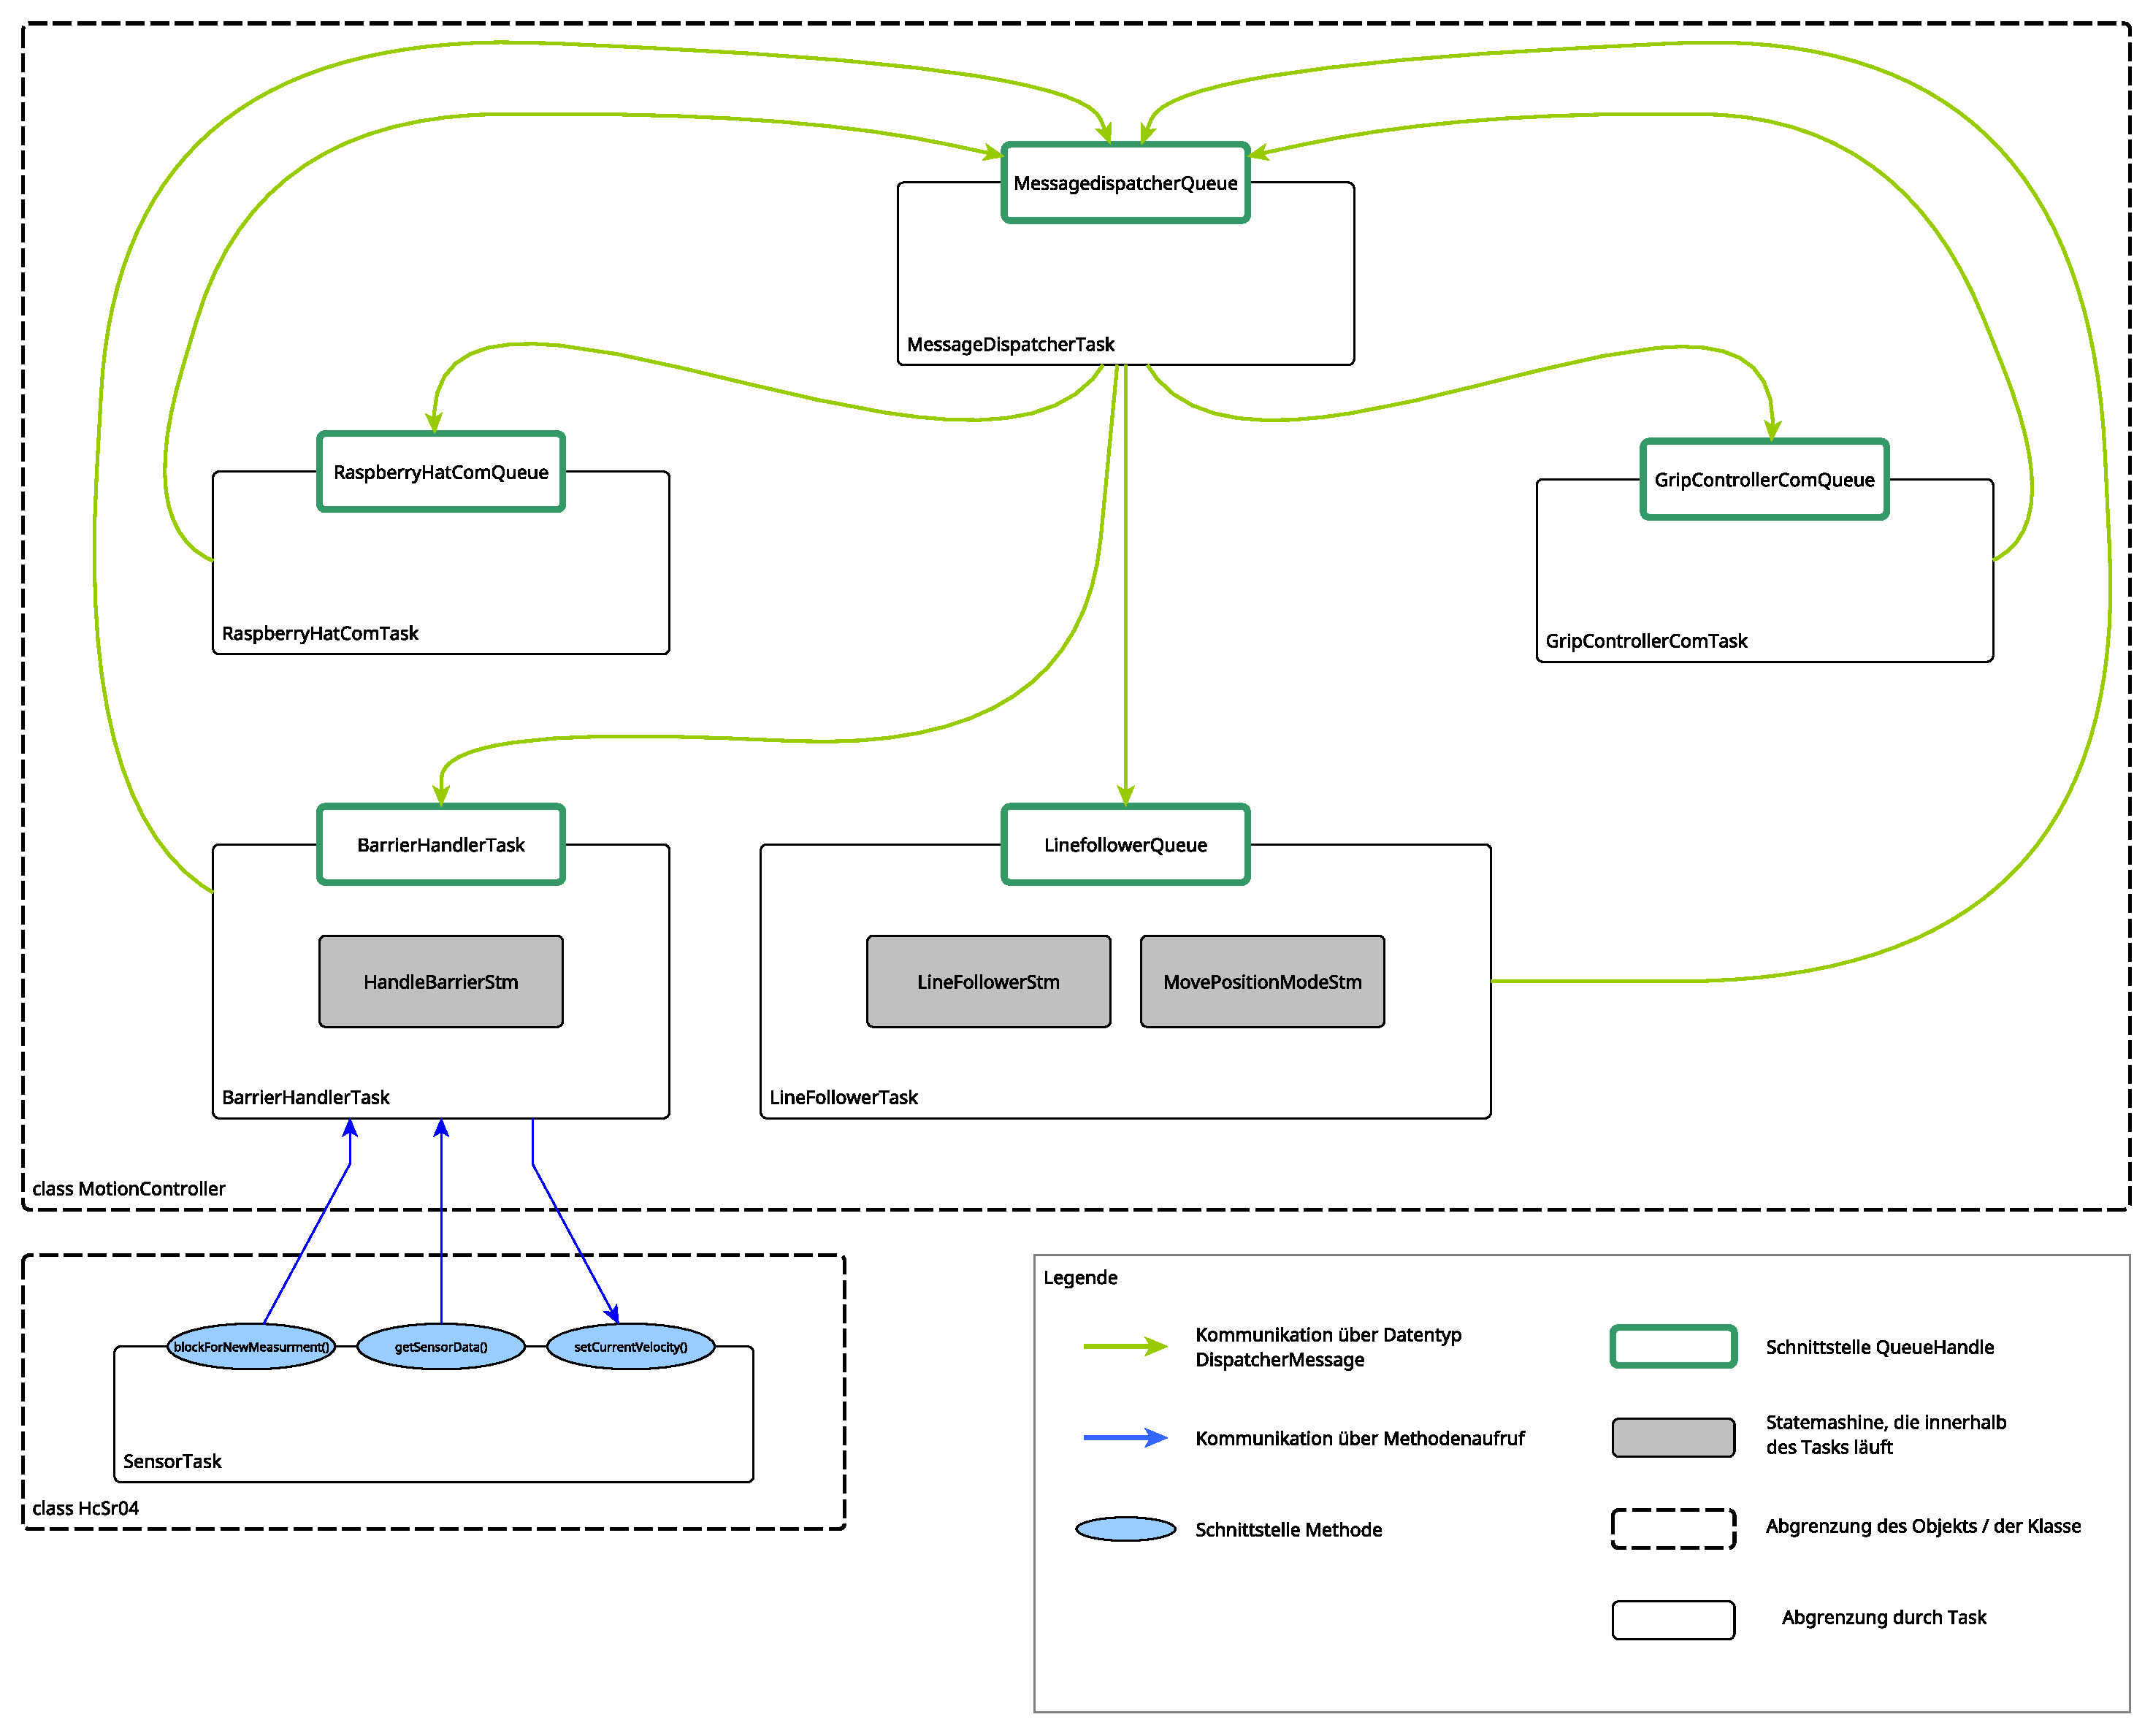
\includegraphics[width=1\linewidth]{./fig_Firmware_MotionController/TaskStruktur.pdf}
    \caption{Struktur der Tasks und der Kommunikation zwischen den tasks}~\ref{fig:TaskStruktur_Motioncontroller}
\end{figure}

\subsubsection*{\texttt{DispatcherMessage}}~\label{apdx:DispatcherMessage}

Dieser Datentyp vereinheitlicht die Kommunikation zwischen den Tasks. Sein
Aufbau ist relativ einfach:

\begin{lstlisting}[language=C++, style=CppStyle, caption={Prototyp DispatcherMessage}]
struct DispatcherMessage
{
    DispatcherTaskId senderTaskId;
    DispatcherTaskId receiverTaskId;
    TaskCommand command;
    uint32_t data[2];
};
\end{lstlisting}

Die Nachricht enthält den Absender, den Empfänger und den zu sendenden Befehl.
Zusätzlich kann ein 64bit Payload an die Nachricht angehängt werden. Dieser
wird verwendet, um beispielsweise im Falle eines \texttt{Move} Kommandos die zu
fahrende Strecke mitzuteilen. Oder im Falle eines \texttt{Turn}-Befehls den zu
fahrenden Winkel.

Die folgende Liste zeigt die möglichen TaskId's:
\begin{description}
    \item[NoTask] Der Standard-Konstruktor setzt diesen Wert.
    \item[Broadcast] Die Nachricht wird an alle Tasks gesendet.
    \item[DispatcherTask] Die Nachricht ist für den MessageDispatcher bestimmt. Diese
        wird noch nicht verwendet.
    \item[LineFollowerTask] Die Nachricht betrifft Bewegungen: der LineFollower wird
        informiert.
    \item[RaspberryHatComTask] Die UART-Schnittstelle zum RaspberryHat wird angesteuert.
    \item[GripControllercomTask] Diese Nachricht soll über UART an den Gripcontroller
        gesendet werden.
    \item[MotionControllerComTask] Hiermit wird die UART Schnittstelle am GripController
        angesprochen.
    \item[ServoDriveTask] Interne Steuerung der Servomotoren auf dem GripController.
    \item[BarrierHandlertask] Interne Bewegungssteuerung des Greifvorgangs auf dem
        MotionController.
\end{description}

Das Feld \texttt{TaskCommand} beschreibt den Befehl, der an die Tasks gesendet
werden soll. Dies kann ein \texttt{Move} oder ein \texttt{Stop} sein, aber auch
Polling-Anfragen des RaspberryHat, die entsprechend beantwortet werden.
Statusinformationen, die an den RaspberryHat gesendet werden, werden mit den
gleichen Kommandos gekennzeichnet. So hat beispielsweise \textit{Knoten
    erkannt} den Befehl \texttt{TaskCommand::NodeDetectedInfo}.

\subsubsection*{LineFollowerTask}
Der LineFollowerTask reagiert auf die folgenden Kommandos:

\begin{description}
    \item[Move] Wenn das Feld \texttt{data} leer ist (= 0), wird \texttt{LineFollowerStm}
        in den Linienfolgemodus versetzt. Ist ein Abstand im
        \texttt{MovePositionModeStm} angegeben, so wird die entsprechende Distanz von
        der \texttt{MovePositionModeStm} abgefahren.
    \item[Stop] Weist \texttt{MovePositionModeStm} an, den Roboter anzuhalten. Es wird
        gewartet, bis das Fahrzeug zum Stillstand gekommen ist und dann eine
        Bestätigung des Stopps über den Befehl \texttt{TaskCommand::PositionReached}
        gesendet. \item[SlowDown] Weist die \texttt{LineFollowerStm} Statemachine an, die
        Geschwindigkeit zu reduzieren. Dies wird verwendet, um die Abtastrate des
        Ultraschallsensors bei Annäherung an ein Hindernis zu erhöhen. \item[Turn] Wie der Name schon sagt, veranlasst dieser Befehl die
        \texttt{MovePositionModeStm} an, den Roboter um den im \texttt{data}-Feld
        angegebenen Winkel zu drehen. Die Winkelangabe erfolgt in $[Grad °] \cdot 10$,
        um die Zahl als Festkommazahl mit einer Nachkommastelle zu übertragen.
\end{description}

Wie bereits erwähnt, steuert diese Task die \texttt{MovePositionModeStm} und
die \texttt{LineFollowerStm} Statemachines. Die \texttt{LineFollowerStm}
implementiert den Regelkreis zum Folgen der Linie.

\subsection*{RaspberryHatComTask}
Dieser Task hat die Hoheit über den \texttt{UART0} Kanal und damit über die
Kommunikation mit dem RaspberryHat. Er übernimmt sowohl das Senden als auch das
Empfangen und Dekodieren von Nachrichten über das \texttt{prain\_uart}
Protokoll.

Er reagiert grundsätzlich nur auf Kommandos in Form von
\texttt{DispatcherMessage} Datenpaketen. Wird eine neue Nachricht über UART
empfangen, wird ein \texttt{UART0\_Rx} Interrupt ausgelöst, der eine
DispatcherMessage mit dem Befehl \texttt{TaskCommand::Decode} in die
Empfangsqueue des RaspberryHatComTasks schickt. Der RaspberryHatComTask kann
dann später diese Nachricht decodieren und an den MessageDispatcher
weiterleiten. Dieser Ablauf ist in Abbildung~\ref{fig:UartAuslesen} nochmals
schematisch dargestellt.

\begin{figure}[H]
    \centering
    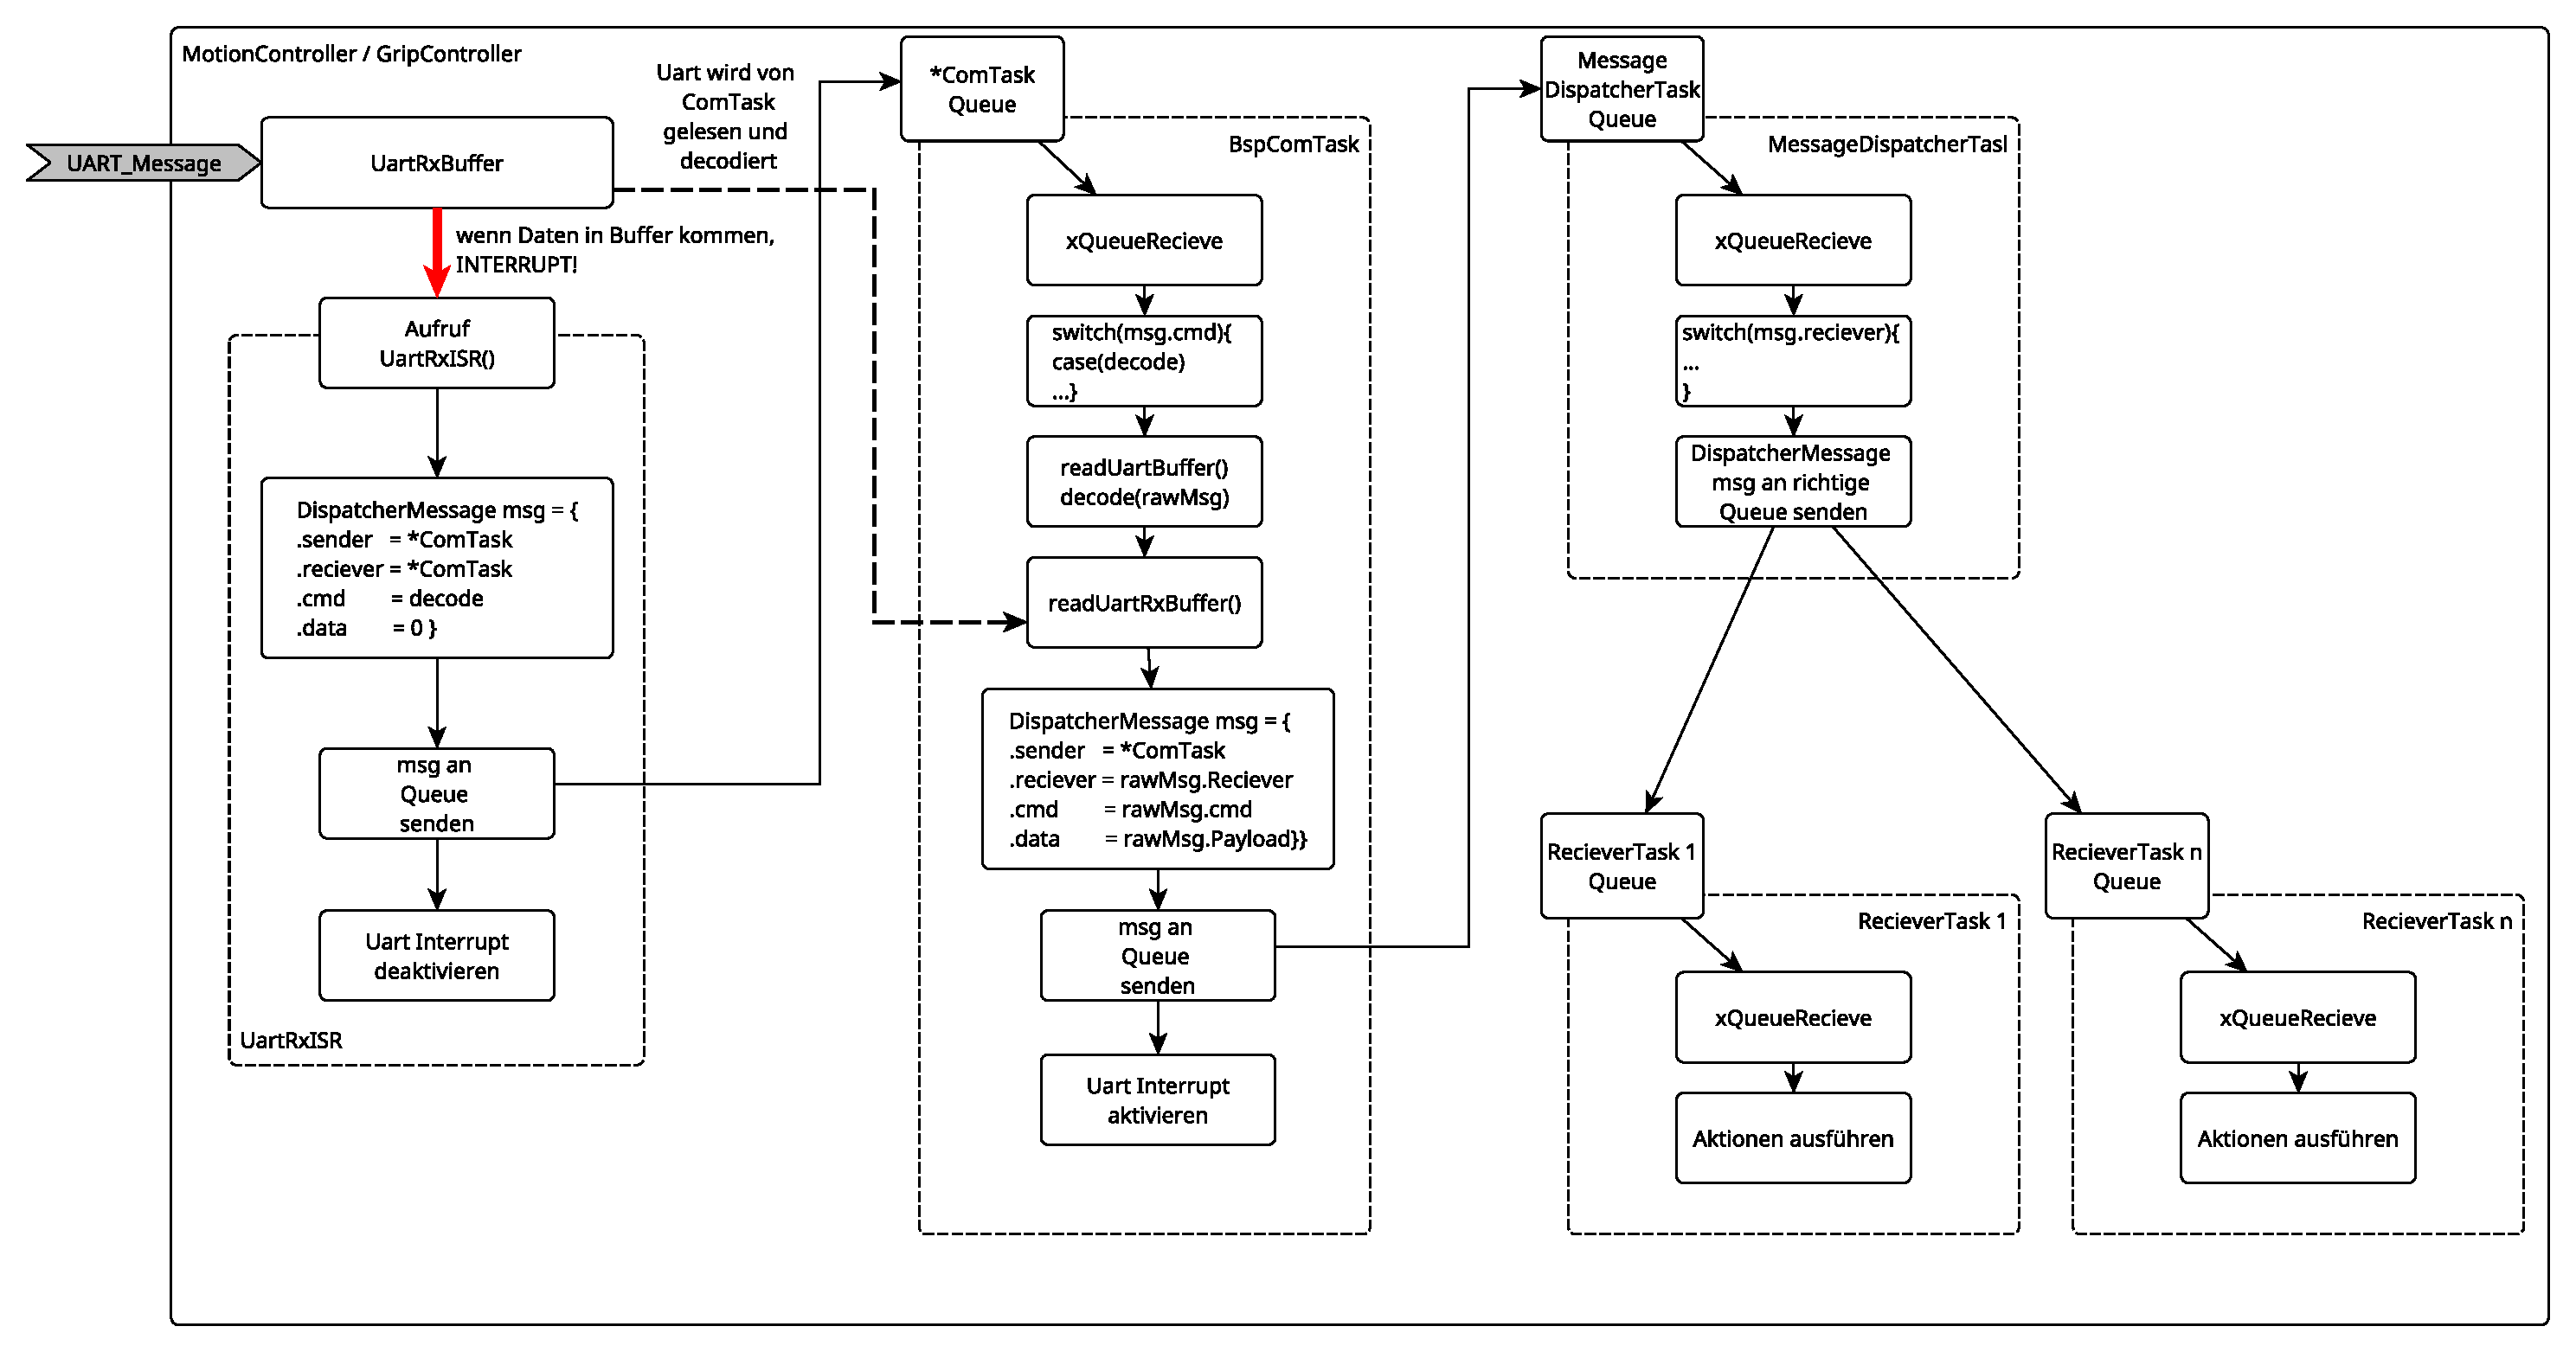
\includegraphics[width=1\linewidth]{./fig_Firmware_MotionController/UartAuslesen.pdf}
    \caption{Auslösung des UART-Interrupts und Kommando geben zum Auslesen}~\label{fig:UartAuslesen}
\end{figure}

Diese Vorgehensweise hat den Vorteil, dass die rechenintensive Decodierung mit
Überprüfung der Prüfsumme nicht innerhalb der Interrupt Service Routine
durchgeführt werden muss.

\subsection*{GripControllerComTask}
Dieser Task übernimmt die gleichen Aufgaben wie der
\texttt{RaspberryHatComTask}, jedoch für die Anbindung des GripControllers über
die \texttt{UART\_1} Schnittstelle.

\subsection*{BarrierHandlerTask}
Dieser Task hat, wie der Name schon sagt, die Hoheit über die Zustandsmaschine,
die den Bewegungsablauf für die Hindernisbehandlung implementiert. Dazu wartet
er auf die Kommandos

\begin{description}
    \item[Move] Startet die Statemachine, die zunächst alle $10ms$ den Abstand zum
        Hindernis überprüft. Über Methodenaufrufe stehen Schnittstellen zur Sensortask
        und damit zum Ultraschallsensor zur Verfügung. Diese Aufrufe sind alle durch
        \texttt{Mutexes} geschützt. Über diese Schnittstellen kann der
        BarrierHandlerTask aktuelle Sensordaten abfragen, die auch aus Vorhersagen
        stammen. Mehr zu diesem Prädiktionsschritt im Anhang \textit{Parametrierung
            HcSr04}.

    \item[Stop] Setzt den Zustnad der Statemaschine zurück auf den \texttt{IDLE} Zustand.

    \item[PositionReached] Signalisiert der Statemaschine, dass die angeforderte Bewegung
        vom LineFollowerTask ausgeführt wurde.
\end{description}

\subsubsection*{Sensortask}
Dieser Task liest nur den Ultraschallsensor aus und führt eine zeitdiskrete Tiefpassfilterung dieser Werte durch.

\subsection{Schnittstelle zum GripController}~\label{apdx:ComGripControllerMotionController}
Im vorherigen Abschnitt wurde der GripController standardmässig über den
\texttt{GripControllerComTask} in das Projekt eingebunden.

Die Instanz des MotionControllers bietet jedoch eine Schnittstelle, die es
erlaubt, den GripController auch als Objektinstanz auf dem MotionController
auszuführen. Dazu muss lediglich der \texttt{GripControllerComTask} durch die
QueueHandles des GripControllers ersetzt werden.

Der GripController arbeitet mit dem gleichen Datentyp
\texttt{DispatcherMessage}, wodurch diese Schnittstelle sehr einfach zu
implementieren ist.

Der MotionController besitzt dazu 2 Methoden, die einerseits den Zugriff auf
den MessageDispatcher erlauben, aber auch das QueueHandle des GripControllers
registrieren. Abbildung~\ref{fig:Einbindung_GripController_als_Instanz} zeigt
noch einmal, wie die Objektinstanz des GripControllers in den MotionController
eingebunden werden kann.

\begin{figure}[H]
    \centering
    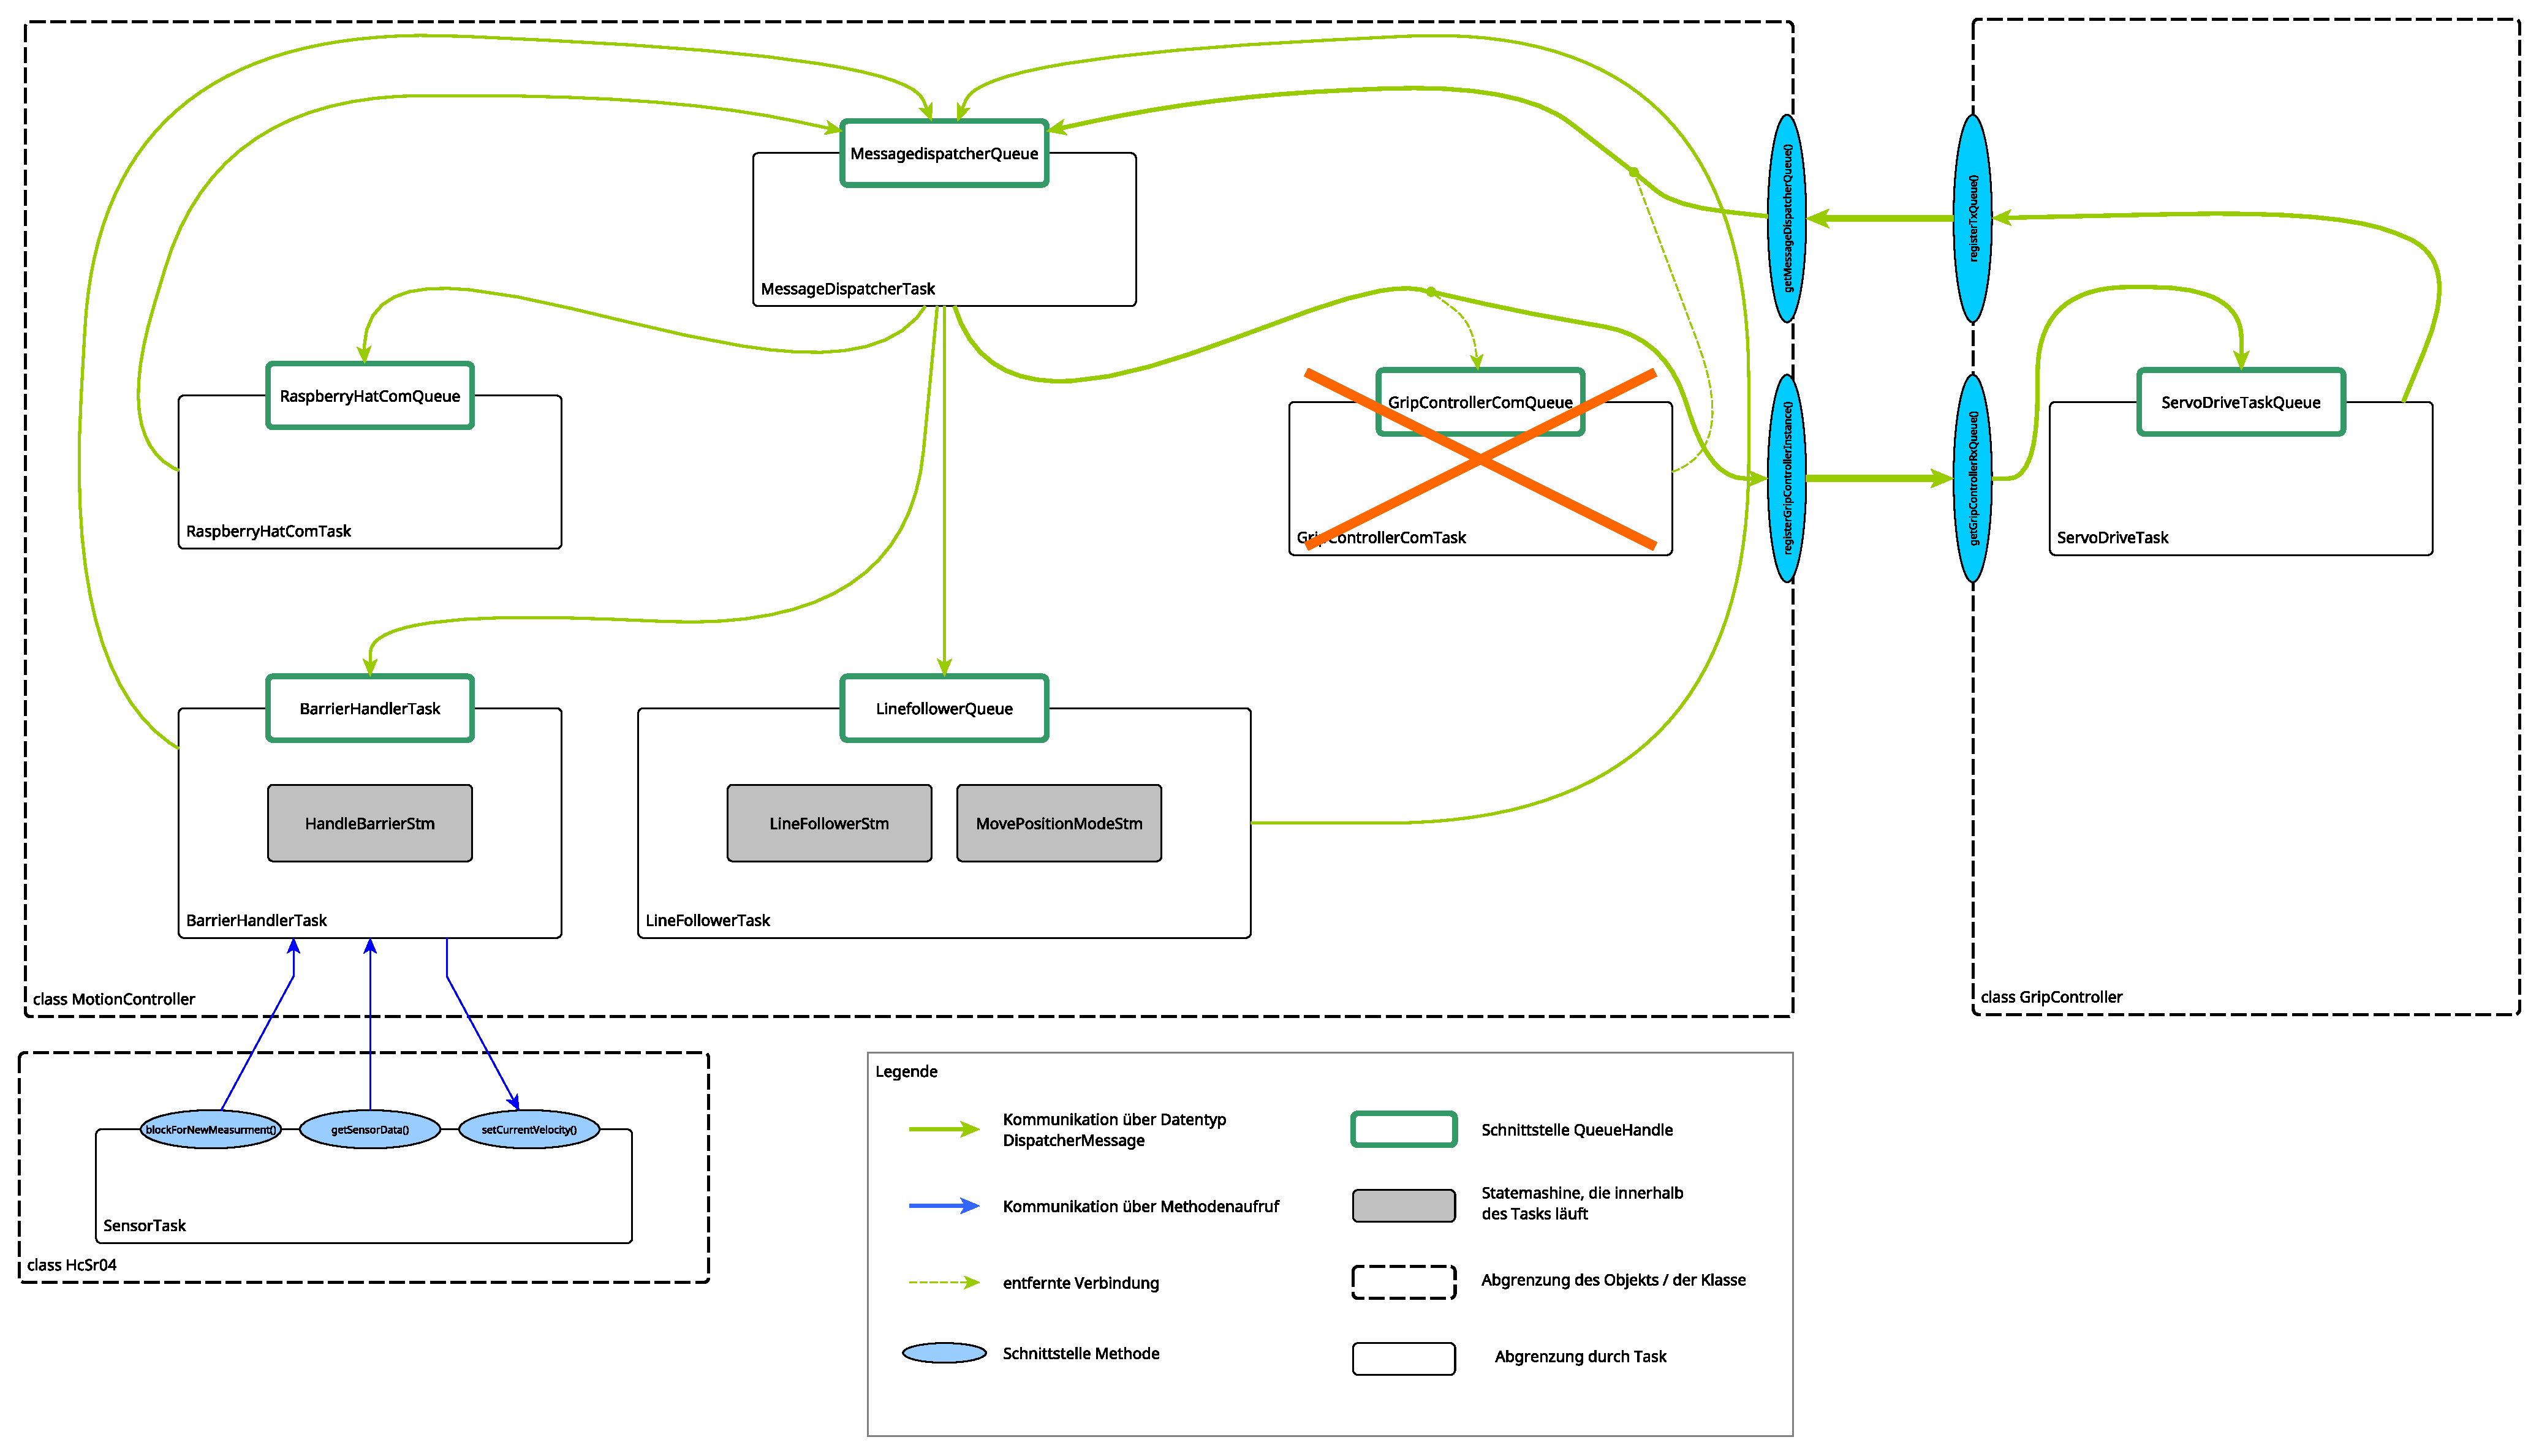
\includegraphics[width=1\linewidth]{./fig_Firmware_MotionController/Einbindung_GripControllerQueues.pdf}
    \caption{Einbindung des GripControllers als Instanz in die Firmware des MotionControllers}~\label{fig:Einbindung_GripController_als_Instanz}
\end{figure}

\subsection{Zustandsmaschinen}
Der folgende Abschnitt beschreibt die verschiedenen Statemachines, die im
MotionController implementiert sind. Bei allen handelt es sich um
Mealy-Automaten. Der Einfachheit halber werden als Stm-Eingänge oft
Pseudofunktionen oder Ausdrücke angegeben, um das entsprechende Eingangssignal
zu benennen. Im Quellcode werden diese häufig durch DispatcheMessages
ausgelöst.

\subsection*{LineFollowerStm}
Diese Statemachine steuert den LineFollower des MotionControllers. Hat der
LineFolger einen Knoten erkannt oder die Linie verloren, wird der Zustand
entsprechend geändert, eine Nachricht an den RaspberryHat gesendet und zurück
in den Idle State gewechselt.

\begin{figure}[H]
    \centering
    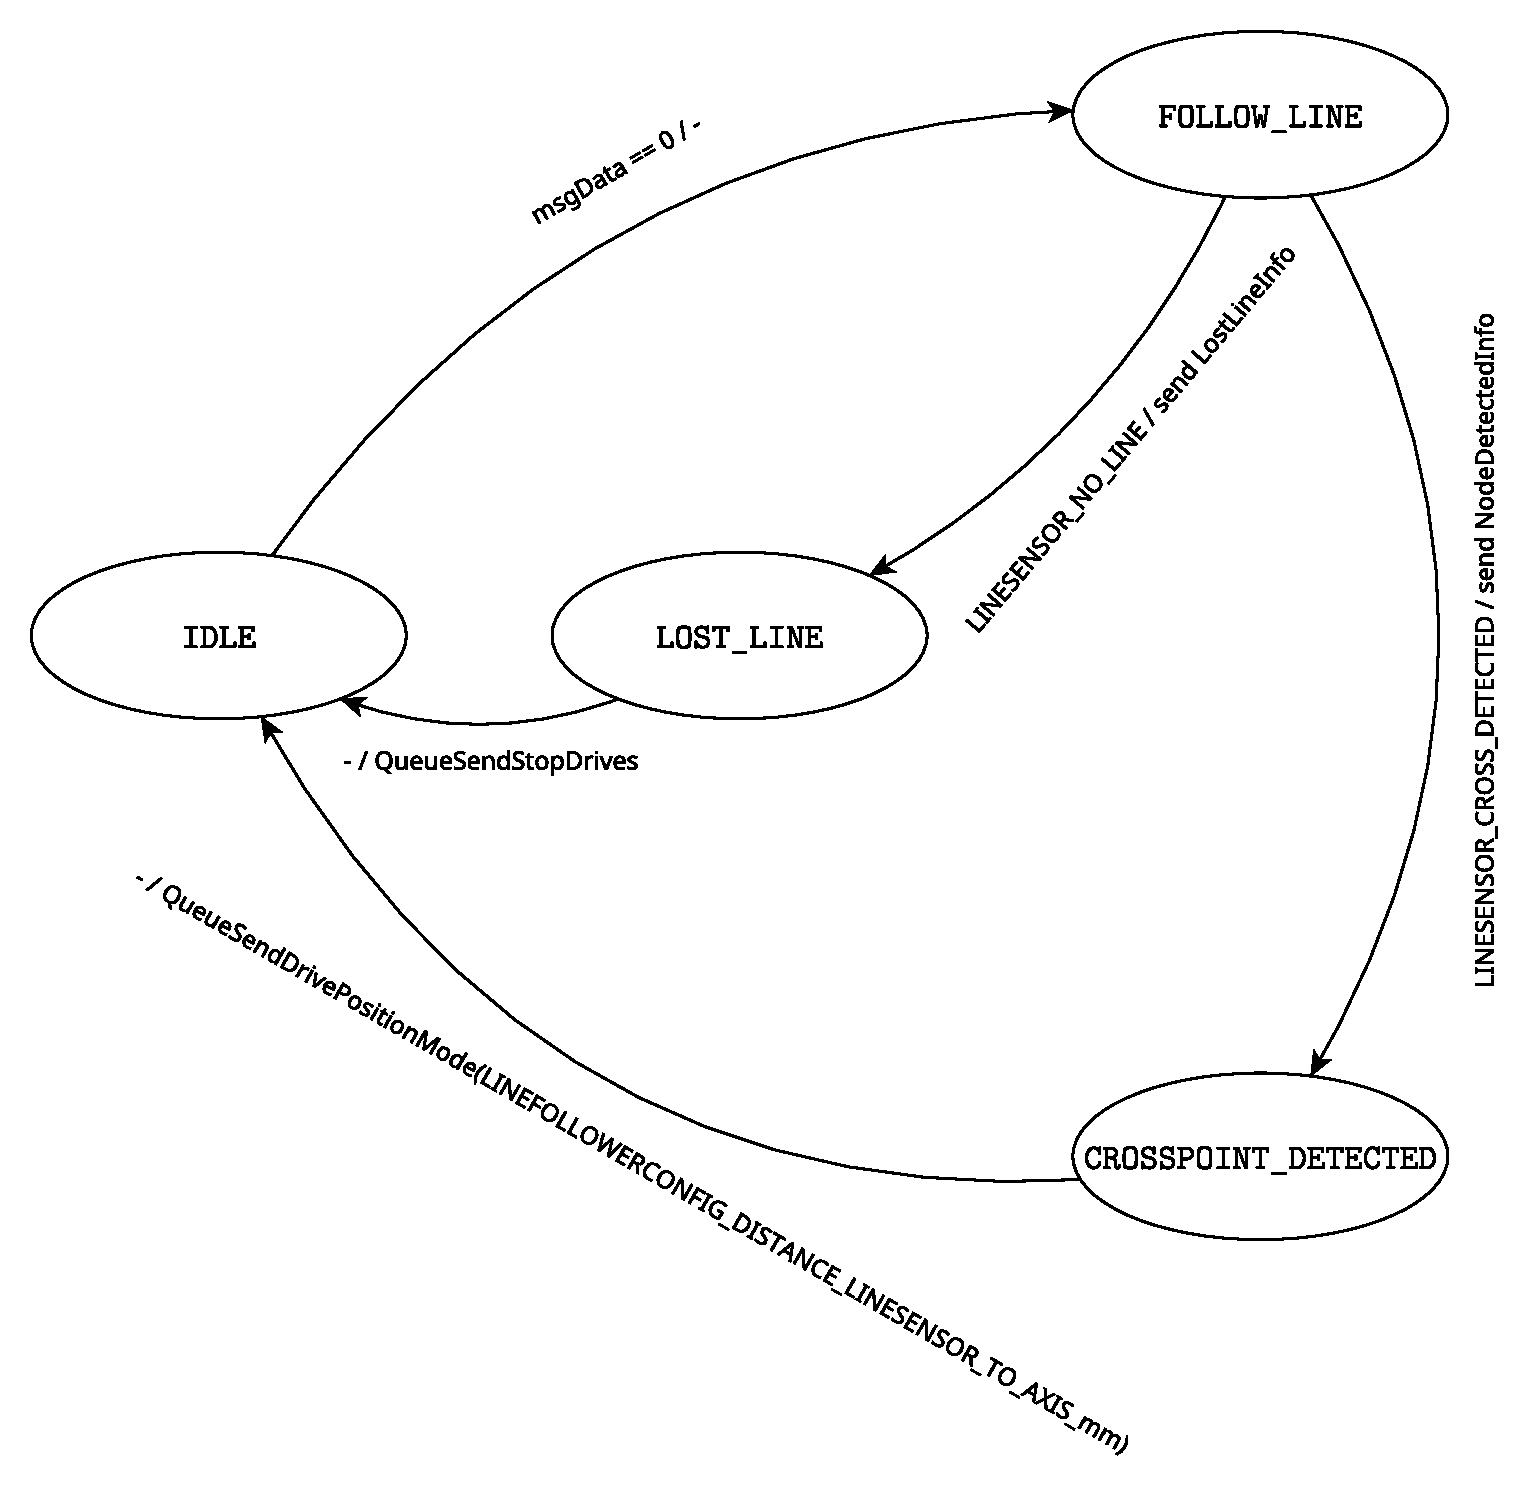
\includegraphics[width=0.75\linewidth]{./fig_Firmware_MotionController/LineFollowerStm.pdf}
    \caption{Zustandsdiagramm LineFollowerStm}~\label{fig:LineFollowerStm}
\end{figure}

Abbildung~\ref{fig:LineFollowerStm} zeigt die verschiedenen Zustände dieser
Zustandsmaschine auf einem Zustandsgraphen auf.

\subsubsection*{MovePositionModeStm}~\label{apdx:MovePositionModeStm}
Die MovePositionModeStm wird ebenfalls vom LineFollowerTask gesteuert. Sie führt manuelle Bewegungen an den Motorentreibern aus.
Konkret geht es dabei um \textit{fahre $[xxx mm]$}, \textit{drehe $[xxx °]$} und auch das Anhalten des Fahrzeugs.

\begin{figure}[H]
    \centering
    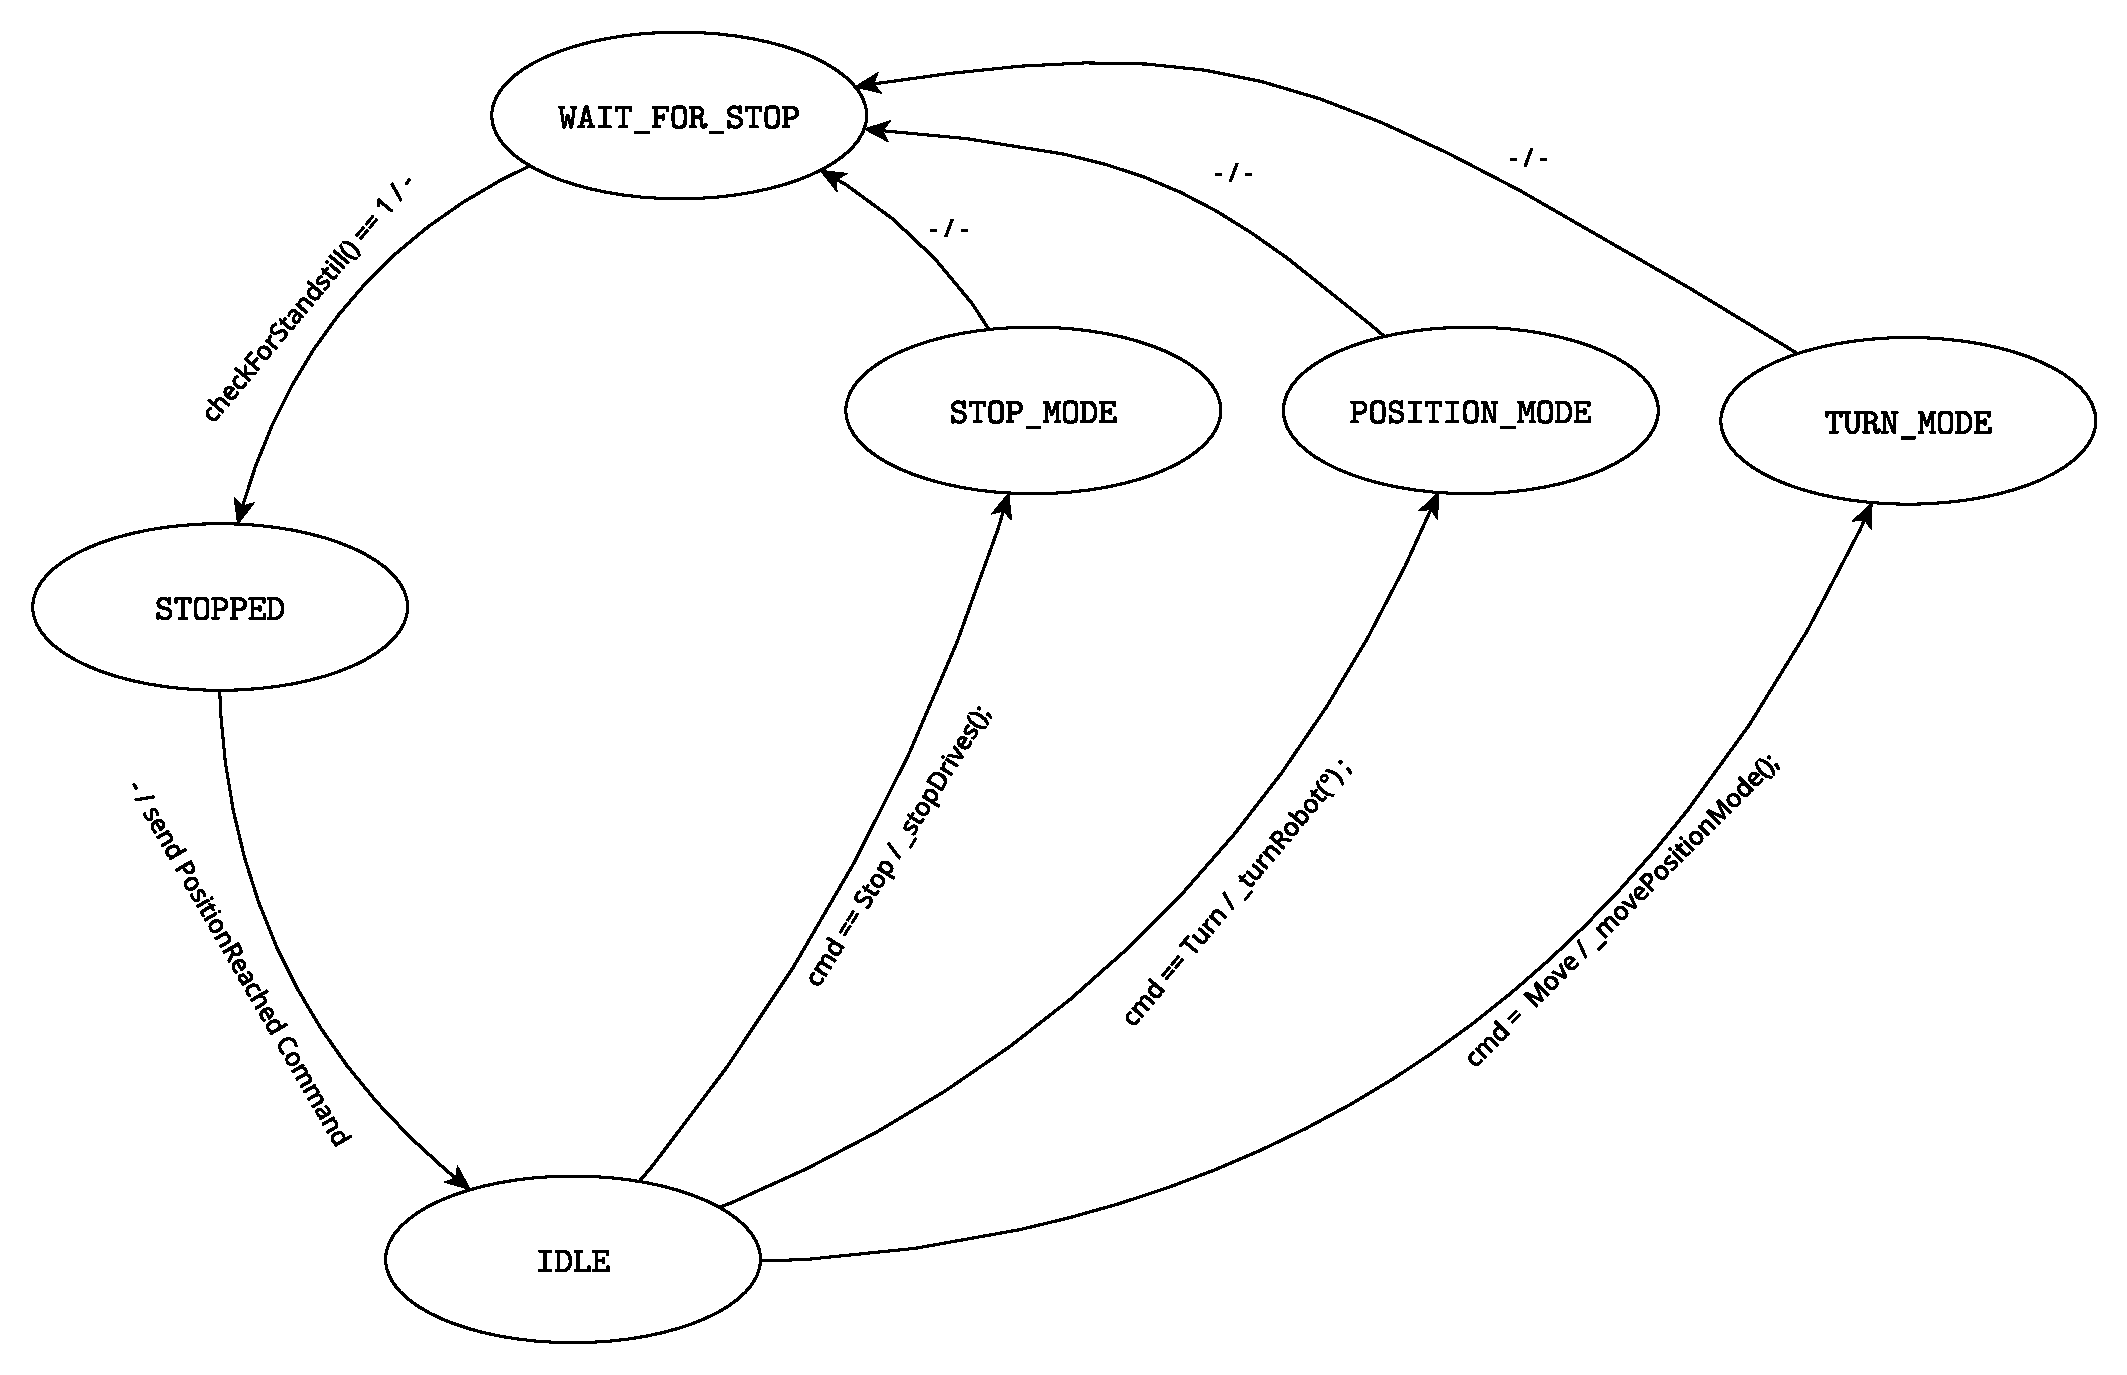
\includegraphics[width=0.75\linewidth]{./fig_Firmware_MotionController/MovePositionModeStm.pdf}
    \caption{Zustandsdiagramm MovePositionModeStm}~\label{fig:MovePositionModeStm}
\end{figure}

Abbildung~\ref{fig:MovePositionModeStm} stellt die verschiedenen Zustände
dieser Zustandsmaschine auf einem Zustandsgraphen dar. Der Übergang von
\texttt{STOP\_MODE}, \texttt{POSITION\_MODE} und \texttt{TURN\_MODE} erfolgt
ohne Eingangssignal.

\subsubsection*{HandleBarrierStm}~\ref{apdx:HandlerBarrierStm}

Die HandleBarrierStm ist die mit Abstand grösste Statemaschine, hat allerdings
auch den komplexesten Bewgungsablauf zu implementieren.

\begin{figure}[H]
    \centering
    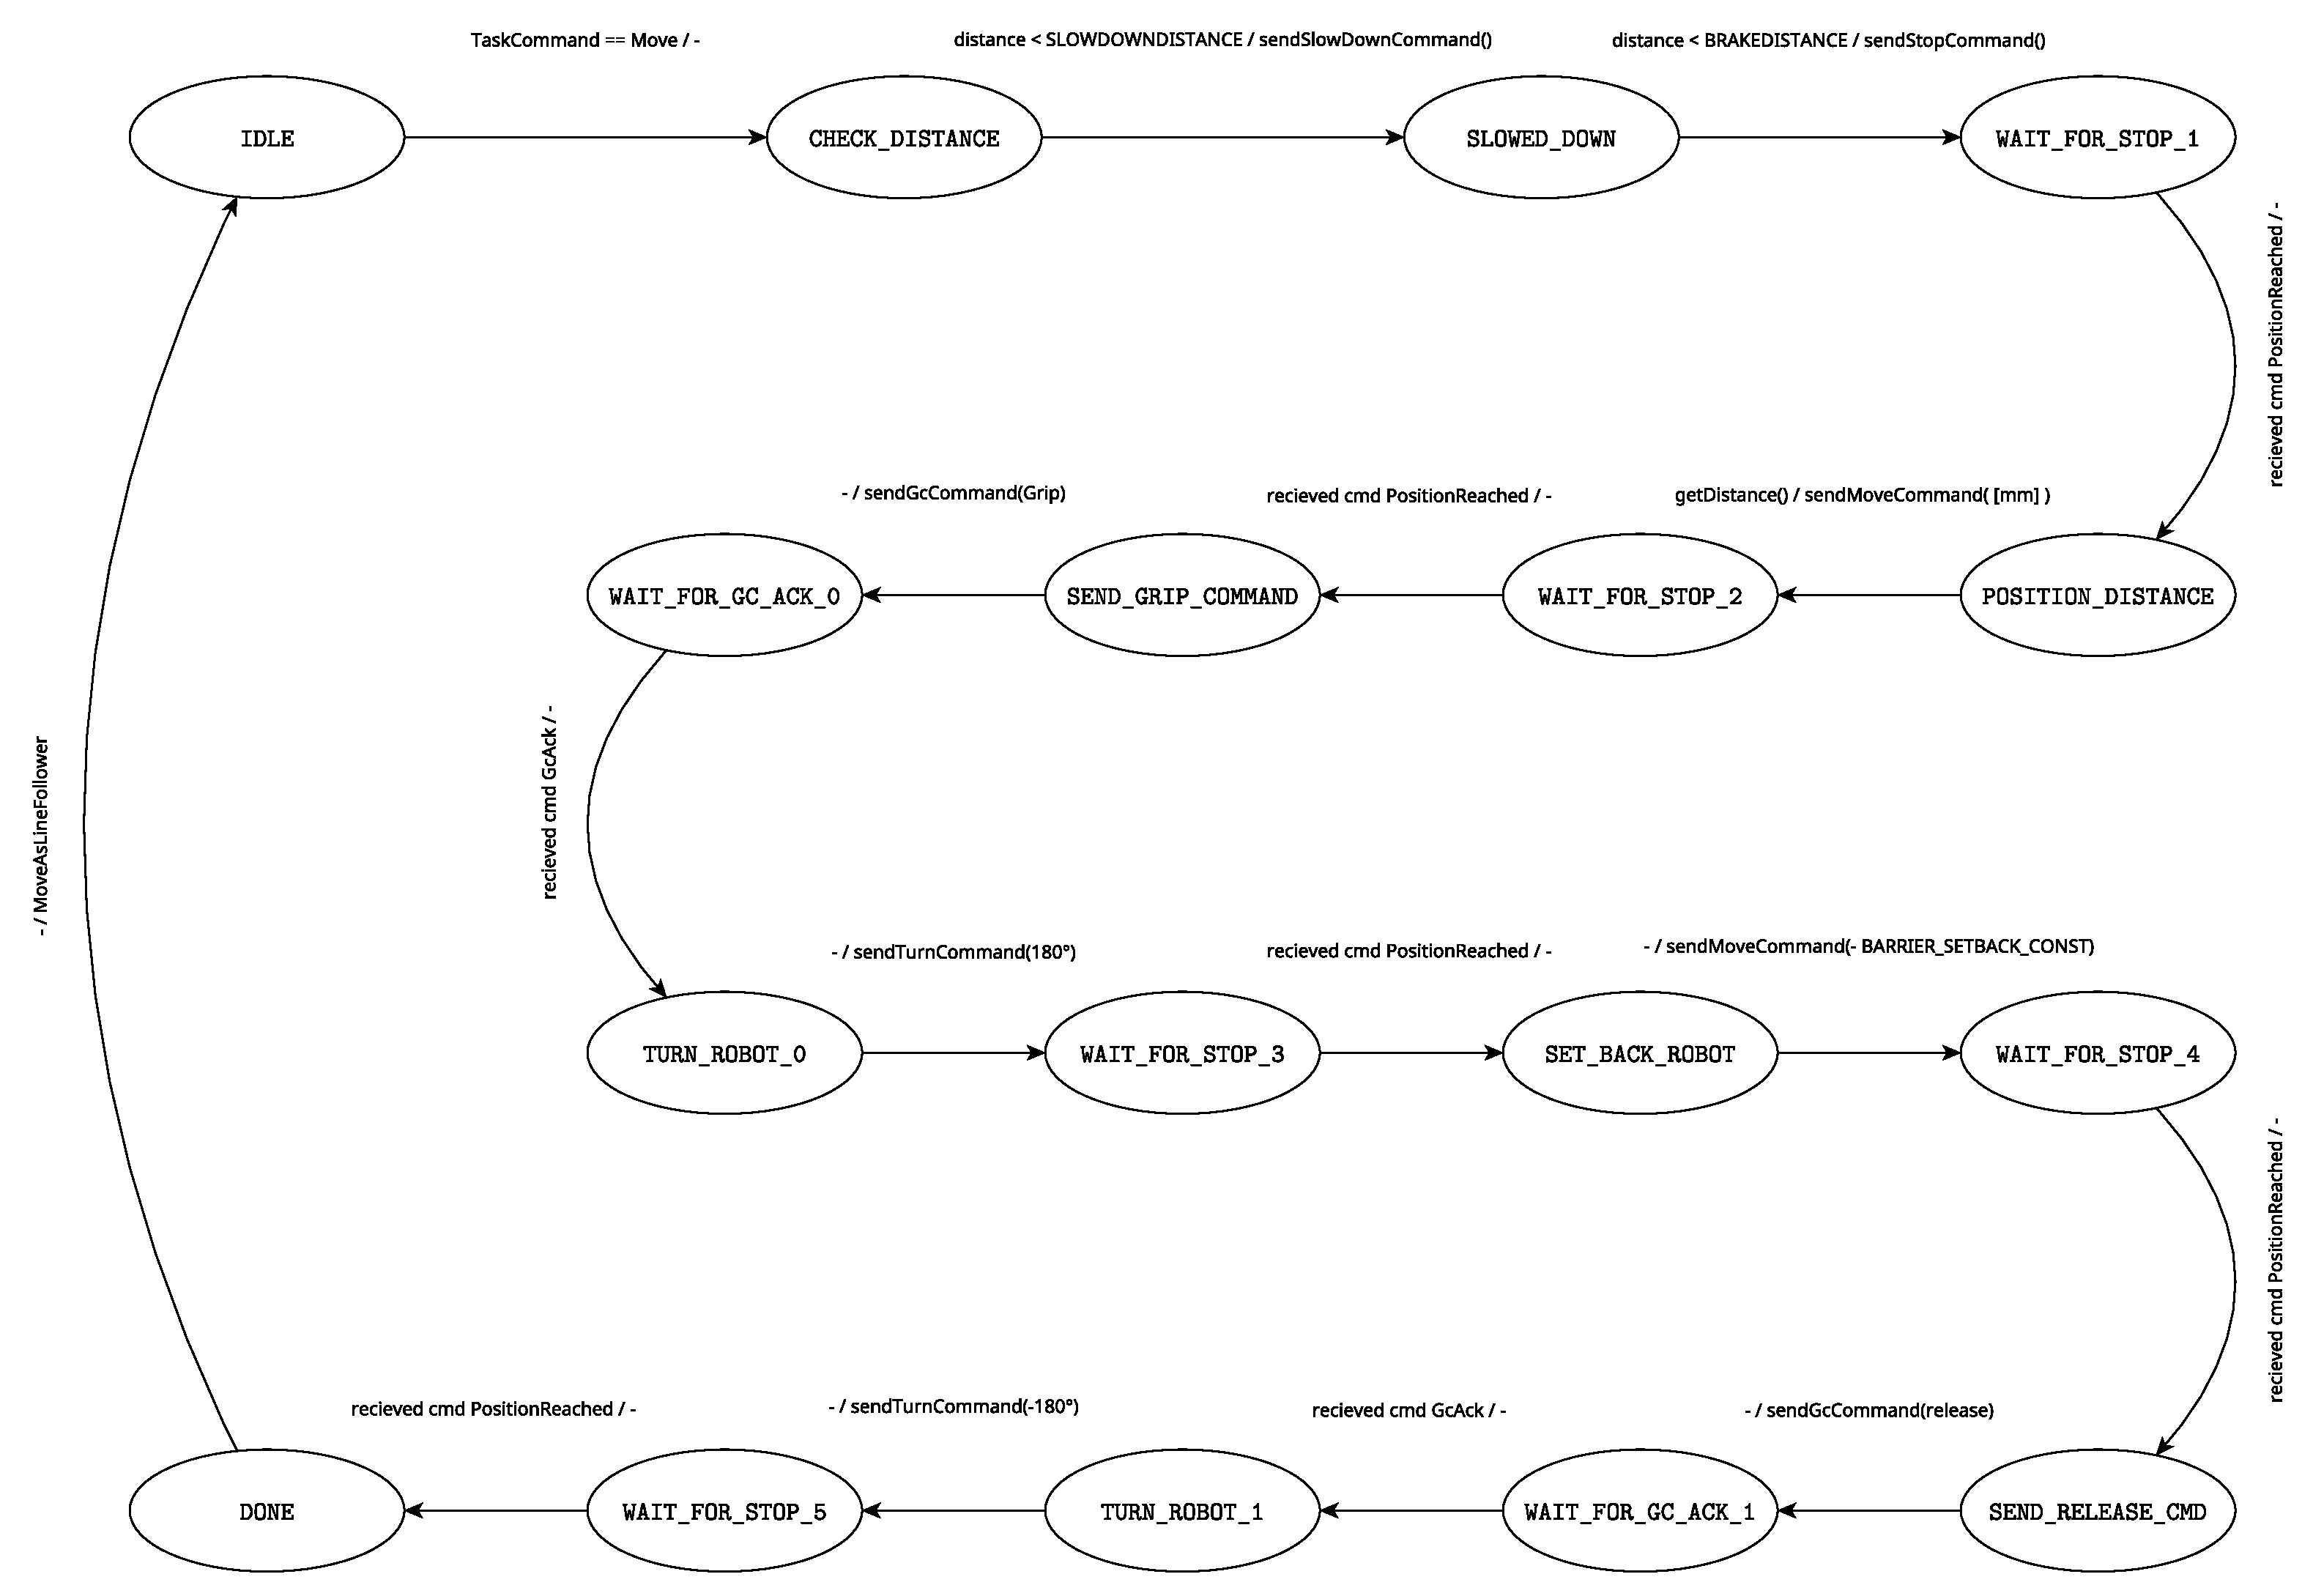
\includegraphics[width=1\linewidth]{./fig_Firmware_MotionController/HandleBarrierStm.pdf}
    \caption{Zustandsdiagramm HandleBarrierStm}~\label{fig:HandleBarrierStm}
\end{figure}

Zuerst wird der aktuelle Abstand zum Hindernis überprüft. Ist dieser kleiner
als ein vorgegebener Bremsweg, wird das Fahrzeug zunächst abgebremst, dann zum
Stillstand gebracht und der Abstand zum Hindernis erneut final korrigiert. Nun
folgt der gesamte Bewegungsablauf, um das Hindernis zu positionieren: Greifen,
Drehen, Rückwärtsfahren, Absetzen, Rückwärtsfahren, Weiterfahren. Dazwischen
gibt es immer wieder Zustände wie \texttt{WAIT\_FOR\_STOP\_X}, die nichts
anderes tun, als auf das Ende der Bewegung zu warten. Diese Zustandsmaschine
wird jedes Mal zurückgesetzt, wenn ein \texttt{Stop}-Kommando empfangen wird.

\subsection{Distanz und Rotation RaspberryHat mitteilen}~\label{apdx:Distanz_Tracking}

Das Konzept sieht vor, dass die zurückgelegte Strecke von RaspberryHat
abgefragt werden kann. Dazu gibt es in der Klasse MotionController ein
MovementTracker Objekt. Diese Kapselung dient zur Speicherung der
Positionsdaten, die aus den Schrittmotortreibern ausgelesen werden können. Die
folgenden Abbildungen zeigen schematisch, wie diese Daten über Distanz und
Winkel vom MotionController verwaltet werden.

\begin{figure}[H]
    \centering
    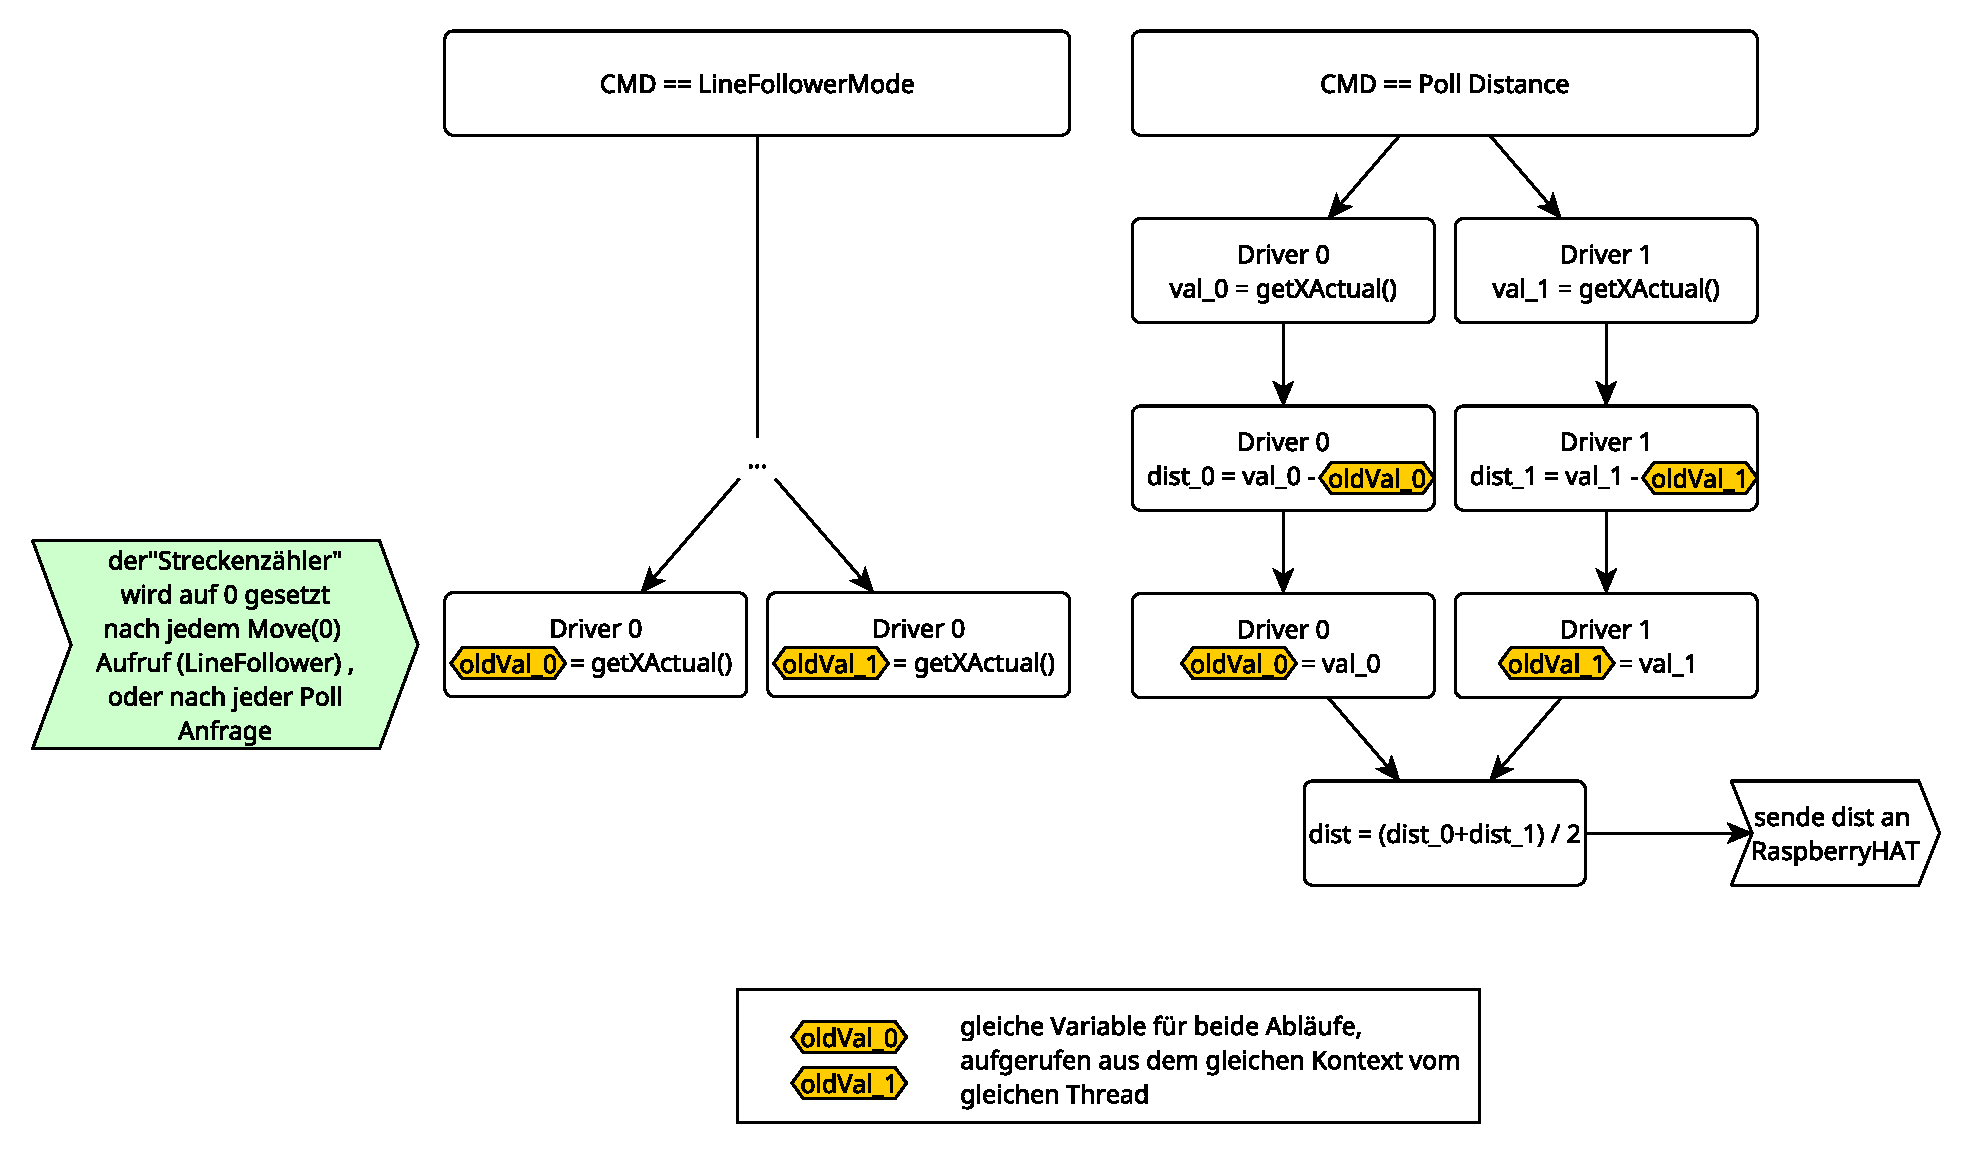
\includegraphics[width=1\linewidth]{./fig_Firmware_MotionController/PollDistance_cmd.pdf}
    \caption{MovementTracker Speichern der Distanz}~\label{fig:MovementTracker_Distanz}
\end{figure}

Abbildung~\ref{fig:MovementTracker_Distanz} zeigt, wie die zurückgelegte
Wegstrecke verwaltet wird. Wurde das Fahrzeug im LineFollowerMode gestartet,
wird der aktuelle Schrittzähler der Schrittmotoren auf 0 gesetzt. Wird zu einem
späteren Zeitpunkt die zurückgelegte Wegstrecke mit einem \texttt{PollDistance}
Befehl abgefragt, so wird der Mittelwert der gelaufenen Schritte beider Motoren
gebildet, der Zähler wieder auf 0 gesetzt und an den RaspberryHat gesendet.

Abbildung~\ref{fig:MovementTracker_Winkel} zeigt, wie die aktuelle Drehung des
Fahrzeugs ermittelt wird. Auch hier wird ein Schrittzähler verwendet, der zu
Beginn auf 0 gesetzt wird.Physikalische Konstanten wie die Achsbreite sind
durch die Fahrzeugstruktur vorgegeben. Aus der Anzahl der Schritte, die jedes
Rad zurückgelegt hat, kann somit direkt auf die Fahrzeugrotation geschlossen
werden.

\end{document}
